
% Preamble
\documentclass[bibliography=totoc, twoside]{article}
\title{\textbf{ThetaNet} \\ A toolkit to simulate networks of Theta Neurons}
\author{Christian Bl\"asche}

% Packages
\usepackage{amsmath, bm}
\usepackage{amsfonts}
\usepackage{todonotes}
\usepackage{float}
\usepackage[linesnumbered,lined,boxed,commentsnumbered, ruled]{algorithm2e}
\usepackage{siunitx}
\sisetup{table-number-alignment=center, exponent-product=\cdot}
\usepackage{booktabs}
\usepackage[hidelinks]{hyperref}
\renewcommand{\subsubsectionautorefname}{subsection}
\renewcommand{\algorithmautorefname}{Algorithm}
\usepackage[margin=1.5in]{geometry}
\usepackage[numbers]{natbib}
\usepackage{graphicx, tabularx, caption}
\usepackage{listings}
\usepackage{xcolor}
\usepackage[onehalfspacing]{setspace}
\setcounter{secnumdepth}{4}
\numberwithin{equation}{section}

\usepackage{fancyhdr}
\fancypagestyle{fance}{
    \fancyhf{}
    \fancyhead[EL]{\nouppercase\rightmark}
    \fancyhead[OL]{\nouppercase\rightmark}
    \fancyfoot[EC,OC]{\thepage}
    \renewcommand{\headrulewidth}{1pt}
}
%\fancypagestyle{plain}{%
%    \fancyhead{} % get rid of headers on plain pages
%    \fancyfoot{} % get rid of headers on plain pages
%    \fancyfoot[EC,OC]{\thepage}
%    \renewcommand{\headrulewidth}{0pt} % and the line
%}


% Own commands
\newcommand{\inn}{\text{in}}
\newcommand{\out}{\text{out}}
\newcommand{\mean}[1]{\left< #1 \right>}
\newcommand{\mk}{\langle k\rangle}
\newcommand{\crossed}{{\backslash \hspace{-4.33pt}/}}
\newcommand{\bk}{{\bm k}}
\newcommand{\be}{\begin{equation}}
\newcommand{\ee}{\end{equation}}
\newcommand*\colvec[1]{\begin{pmatrix}#1\end{pmatrix}}
\newenvironment{rcases}
  {\left.\begin{aligned}}
  {\end{aligned}\right\rbrace}




\begin{document}

\maketitle
\vspace{1.7in}
\tableofcontents
\thispagestyle{empty}

\newpage
\pagestyle{fance}
\definecolor{codegreen}{rgb}{0,0.6,0}
\definecolor{codegray}{rgb}{0.5,0.5,0.5}
\definecolor{codepurple}{rgb}{0.58,0,0.82}
\definecolor{backcolour}{rgb}{0.98,0.98,0.95}

\lstdefinestyle{mystyle}{
    backgroundcolor=\color{backcolour},
    commentstyle=\color{codegreen},
    keywordstyle=\color{blue},
%    numberstyle=\tiny\color{codegray},
    stringstyle=\color{codepurple},
    basicstyle=\ttfamily\footnotesize,
    breakatwhitespace=false,
    breaklines=true,
    captionpos=b,
    keepspaces=true,
%    numbers=left,
%    numbersep=5pt,
    showspaces=false,
    showstringspaces=false,
    showtabs=false,
    tabsize=2
}
\lstset{style=mystyle}

\section{Miscellaneous}

\textit{ThetaNet} is a Python3 module comprising the following features:
\begin{itemize}
\item Create correlated (Gaussian copula) and uncorrelated degree sequences
\item Create and adjacency matrices, remove self- and multi-edges, and manipulate degree assortativity
\item Integrate networks of theta neurons
\item Integrate degree mean field dynamics of theta neuron networks
\item Numerically continue solutions with respect to coupling strength, intrinsic excitability, and degree correlation/assortativity
\end{itemize}
It is published under the GNU General Public License v2.0.

\subsection*{Installation}
If you do not have python3 installed yet, get it from \url{https://www.python.org/downloads/}.
\begin{itemize}
    \item Install the package \textit{setuptools} from \url{https://pypi.org/project/setuptools/} or if you have the \textit{pip} installed run:
\begin{lstlisting}[language=Bash]
pip3 install setuptools
\end{lstlisting}
    \item Download the repository from \url{https://github.com/cblasche/thetanet} or if you have \textit{git} installed run:
\begin{lstlisting}[language=Bash]
git clone https://github.com/cblasche/thetanet
\end{lstlisting}
    \item In the same folder as above run:
\begin{lstlisting}[language=Bash]
python3 setup.py install
\end{lstlisting}
\end{itemize}


\subsection*{Structure}
\begin{itemize}
    \item \textbf{thetanet.dynamics} contains differential equations and integrator setup for a network of Theta neurons, the ensemble equations and the mean field equations.
    \item \textbf{thetanet.generate} holds functions to generate degree sequences, adjacency matrices and assortativity functions. Additionally, there are functions to compute degree correlations and assortativity coefficients.
    \item \textbf{thetanet.continuation} stores various continuation schemes.
    \item \textbf{thetanet.utils} has functions around the topics: correlated probability function, polynomial chaos expansion, and singular value decomposition.
\end{itemize}


\subsection*{Parameter file}
Due to the larger number of parameters, functions related to the dynamics, i.e.\ time integration or continuation, require a parameter file.
For convenience, the file is chosen to be a python file, for example the file found in the repository ``example/parameters.py''.
If stored in the same folder as your main script import it and optionally give it a short name with
\begin{lstlisting}[language=python]
import parameters as pm
\end{lstlisting}
We can now pass all parameters at once to a function and access single parameters using the ``dot''-operator.
\begin{lstlisting}[language=python]
def f(pm):
    print("Number of neurons:", pm.N)
\end{lstlisting}
This example illustrates that variable names in the parameter file have to match the specific ones used in the ThetaNet module.
Those names can be found when inspecting the source code or in the example parameter file.
Often it is feasible to alter parameters throughout your execution script, which can be done as simple as:
\begin{lstlisting}[language=python]
pm.N = 1000
f(pm)
# >>> Number of neurons: 1000

pm.N = 2000
f(pm)
# >>> Number of neurons: 2000
\end{lstlisting}


\section{Theta neurons}
We consider a network of $N$ theta neurons:
\be
   \frac{d\theta_i}{dt}=1-\cos{\theta_i}+(1+\cos{\theta_i})(\eta_i+I_i) \label{eq:dthetadt}
\ee
for $i=1,2,\dots N$ where
\be
   I_i=\frac{\kappa}{\mk}\sum_{j=1}^NA_{ij}P_n(\theta_j) \label{eq:I}
\ee
$\eta_i$ is a constant current entering the $i$th neuron, randomly chosen from a distribution
$g(\eta)$, $\kappa$ is strength of coupling,
$\mk$ is mean degree of the network, and the connectivity of the network is given by
the adjacency matrix $A$, where
$A_{ij}$ equals the number of connections between from neuron $j$ to neuron $i$; it may be zero.
A neuron is said to fire when $\theta$
increases through $\pi$, and the function
\be
   P_n(\theta)=d_n(1-\cos{\theta})^n; \qquad n\in\{2,3,\dots\} \label{eq:pq}
\ee
 in~\eqref{eq:I} is meant to mimic the current pulse injected from neuron $j$ to any postsynaptic neurons when
neuron $j$ fires. $d_n$ is a normalisation constant such that $\int_0^{2\pi}P_n(\theta)d\theta=2\pi$
independent of $n$.
\\
For the degree mean field we will assume that the function $g(\eta)$ is a Lorentzian
\be
   g(\eta)=\frac{\Delta/\pi}{(\eta-\eta_0)^2+\Delta^2}
\ee
as this enables us to make use of the Ott/Antonsen ansatz~\cite{ott2008low}.
A degree $\bk$ in a directed network is the tupel $(k^\inn, k^\out)$ and thus we write for the dynamical equations
\be
  \frac{db_\bk}{dt}=\frac{-i(b_\bk-1)^2}{2}+\frac{(b_\bk+1)^2}{2}\left[-\Delta+i\eta_0+i \tilde{I}_\bk\right] \label{eq:b_dbdt}
\ee
where the mean field equivalent of a synaptic current reads
\be
    \tilde{I}_\bk=\frac{\kappa}{\mean{k}}\sum_{\bk^\prime} Q_{\bk \bk^\prime} \tilde{P}_n(b_{\bk^\prime})  \label{eq:Jb}
\ee
and the mean field current pulse
\be
   \tilde{P}_n(b_\bk)=d_n\left[\Gamma_0+\sum_{p=1}^n \Gamma_p(b_\bk^p+c.c.)\right]
\ee
with \textit{c.c.} indicating the complex conjugate and normalisation factors
\be
   \Gamma_p=\sum_{k=0}^n\sum_{m=0}^k\frac{\delta_{k-2m,p}n!(-1)^k}{2^k(n-k)!m!(k-m)!}
\ee

There are two versions of effective degree connectivity $Q_{\bk \bk^\prime}$.
The first is utilised in~\cite{chandra2017modeling, laing2019} and has the form
\be
Q_{\bk \bk^\prime} = P_\bk a(\bk'\rightarrow \bk)
\ee
Note that $P_\bk$ is the probability of a randomly chosen node of the network to have the degree $\bk$, it is not related to the current pulse $P_n(\theta)$ nor to the mean field current pulse $\tilde{P}_n(\bk)$.
It is normalised $\sum_\bk P_\bk = 1$.
The function $a(\bk'\rightarrow \bk)$ is the conditional probability of degree $\bk'$ being connected to degree $\bk$ given their degrees. Note that this probability is not symmetric. With $\alpha, \beta \in [\inn, \out]$ the function can model ($\alpha,\beta$)-degree assorativity to some extent
\be
a(\bk'\rightarrow \bk) = \frac{k_{\inn} k_{\out}^\prime + c\cdot \Big(k_{\alpha} - \left<k_\alpha \right> \Big)\left(k_{\beta}^\prime - \left<k_\beta^\prime \right> \right)   }{N \left<k\right>}
\ee
with $c$ being an assortativity tuning parameter.
The mean values $\left<k_\alpha \right>$ are to be taken over all edges of the network, where $k_\alpha$ means all receiving $\alpha$-degrees and $k^\prime_\beta$ are the $\beta$-degrees of sending nodes.

In the second approach~\cite{blasche2019} transforms we transform an actual adjacency matrix $A_{ij}$ in a degree connectivity matrix $E_{\bk \bk^\prime}$ as follows
\begin{align}
    Q_{\bk \bk'} &= E_{\bk \bk'} \\
    &= C_{\bk i} A_{ij} B_{j \bk'}
\end{align}
with $C$ and $B$ constructed based on the knowledge of $A$ to average nodes sharing the same degree.
\\
More theoretical background is provided in the authors thesis.


\section{thetanet.generate}
\paragraph*{Sequences}
Suppose we would like to create degree squences for $N$ neurons from a given degree space and distribution with a certain degree correlation $\rho$.
We write
\begin{lstlisting}[language=python]
# modules
import numpy as np
import thetanet as tn

# degree space
k_in = np.arange(200, 400)
k_out = np.copy(k_in)

# marginal power law degree distribution
P_k_in = k_in.astype(float)**(-3)
P_k_in /= P_k_in.sum()
P_k_out = np.copy(P_k_in)

# correlated degree distribution
rho = 0.4
P_k_func = tn.utils.bivar_pdf_rho(k_in, P_k_in, k_out, P_k_out)
P_k = P_k_func(rho)

# degree sequences
N = 1000
K_in, K_out = tn.generate.degree_sequence_copula(P_k, N, k_in, k_out)
\end{lstlisting}

\paragraph*{Configuration model}
Having the sequences one can generate adjacency matrices employing the configuration model.
Consider a simple network with no self- and multi-edges and (in,out) assortativity.
The convention is that an edge $A_{ij}$ is directed from neuron $j$ to neuron $i$.
Degree assortativity of type (in,out) means correlation between the properties in-degree of the sending neuron ($j$) and out-degree of the receiving neuron ($i$);
hence the ThetaNet naming \texttt{j\_prop} and \texttt{i\_prop}.
\begin{lstlisting}[language=python]
# for a simple network
A = tn.generate.configuration_model(K_in, K_out)

# for a network containing self- and multi-edges
A = tn.generate.configuration_model(K_in, K_out, simple=False)

# for a simple assortative network
r = 0.3
j_prop = 'in'
i_prop = 'out'
A = tn.generate.configuration_model(K_in, K_out, r, i_prop, j_prop)
\end{lstlisting}
Internal operations can also be called explicitly on an existing matrix $A$.
\begin{lstlisting}[language=python]
tn.generate.remove_self_edges(A)
tn.generate.remove_multi_edges(A)
tn.generate.assortative_mixing(A, r, i_prop, j_prop)

# assortative mixing will create multi-edges, which can also be kept
tn.generate.assortative_mixing(A, r, i_prop, j_prop, eliminate_multi_edges=False)
\end{lstlisting}

\paragraph*{Chung-Lu model}
We can also employ the Chung-Lu model.
To achieve a non-vanishing assortativity, we either perturb the target connection probabilities with a parameter $c$ or create a neutral network and apply the mixing algorithm.
\begin{lstlisting}[language=python]
# perturb connectivity probability
c = 2
A = tn.generate.chung_lu_model(K_in, K_out, c, i_prop, j_prop)

# apply mixing algorithm
A = tn.generate.chung_lu_model(K_in, K_out)
tn.generate.assortative_mixing(A, r, i_prop, j_prop)
\end{lstlisting}

\paragraph*{Measures}
There are functions implemented to compute the degree correlation $\rho$ and the assortativity coefficient $r$ from matrices and sequences.
\begin{lstlisting}[language=python]
# degree correlation rho
rho = tn.generate.rho_from_sequences(K_in, K_out)
rho = tn.generate.rho_from_matrix(A)

# assortativity coefficient r
r = tn.generate.r_from_matrix(A, i_prop, j_prop)
\end{lstlisting}

\paragraph*{Assortativity function}
ThetaNet supports three different approaches when computing degree mean field equations where each requires a different assortativity function.
\begin{enumerate}
    \item The assortativity function of the authors of~\cite{chandra2017modeling} depends on the assortativity parameter $c$ and utilizes the full degree space.
\begin{lstlisting}[language=python]
a = tn.generate.a_func_linear(k_in, k_out, P_k, N, c, i_prop, j_prop)
# or without assortativity
a = tn.generate.a_func_linear(k_in, k_out, P_k, N)
\end{lstlisting}

    \item In case of large degree spaces it may be useful to coarse-grain the degree space first and simulate a network of virtual degrees of size $N_{\mu_\inn}\times N_{\mu_\out}$.
    This approach additionally requires the degree probability of those virtual degrees as well as weights to accurately approximate sums over the degree space.
\begin{lstlisting}[language=python]
# virtual degrees and their weights
N_mu_in = 10
k_v_in, w_in, q_in = tn.utils.three_term_recursion(N_mu_in, k_in, P_k_in)
k_v_out, w_out = np.copy((k_v_in, w_in))
w = np.outer(w_in, w_out)

# virtual degree distribution
import scipy.interpolate as si # required for 2d interpolation
P_k_v_func = lambda rho: si.interp2d(k_in, k_out, P_k_func(rho))(k_v_in, k_v_out)
P_k_v = P_k_v_func(rho)

# virtual degree space: assortativity function
a_v = tn.generate.a_func_linear(k_v_in, k_v_out, w*P_k_v, N, c, i_prop, j_prop)
\end{lstlisting}

    \item The third approach is used in~\cite{blasche2019}, where the adjacency matrix $A$ is transformed by matrix multiplication into $E=CAB$.
    Here, introducing degree clusters can be a favourable option when dealing with large degree spaces.
    The amount of clusters are $N_{c_\inn}$ and $N_{c_\out}$.
    There are two implemented ways to create the binning of the degree space, either ``linear'' or using the cumulated sum of the degree probability (``cumsum'').
\begin{lstlisting}[language=python]
N_c_in, N_c_out = 10, 10
E, B, c_in, c_out = tn.generate.a_func_transform(A, N_c_in, N_c_out, mapping='cumsum')
\end{lstlisting}
    The variables \texttt{c\_in} and \texttt{c\_out} are representative degrees of the respective cluster.
\end{enumerate}


\section{thetanet.dynamics}
\paragraph*{Full neuronal model}
Suppose we want to integrate the full Theta neuron model, where each neuron gets assigned a node in the network.
The parameter file requires the definition of $A$ and $N$ as well as the following variables:
\begin{lstlisting}[language=python]
# coupling strength
kappa = 3

# pulse function
n = 2  # sharpness parameter
d_n = 2 ** n * (np.math.factorial(n)) ** 2 \
      / float(np.math.factorial(2 * n))  # normalisation factor
Gamma = tn.dynamics.degree_network.Gamma(n)  # ensemble coefficients

# eta's drawn from Lorentzian (Cauchy) distribution
from scipy.stats import cauchy
eta_0 = -2  # center of distribution
delta = 0.1  # width of distribution
eta = cauchy.rvs(eta_0, delta, size=N)

# time
t = np.linspace(0, 30, 1000)
\end{lstlisting}
After having defined all parameters in parameters.py we simply call:
\begin{lstlisting}[language=python]
import thetanet as tn
import paramters as pm

# start from uniformly distributed angles
theta_t = tn.dynamics.node_network(pm)  # axis 0: time, axis 1: neurons

# start from last time step
theta_t = tn.dynamics.node_network(pm, init=theta_t[-1])

# integrate ensemble equations
z_t = tn.dynamics.node_network_mean(pm)
\end{lstlisting}


\paragraph*{Degree mean field}
The degree mean field can be computed utilizing one of three approaches related to the respective assortativity function.
\begin{enumerate}
    \item Additionally, for a full degree space integration the parameter file has to contain the assortativity function \texttt{a} and degree probability \texttt{P\_k}:
\begin{lstlisting}[language=python]
import thetanet as tn
import parameters as pm  # parameter file additionally requires: a, P_k

pm.degree_approach = 'full'

# start from zero
b_t = tn.dynamics.degree_network.integrate(pm)  # axis 0: time, axis 1: degrees

# start from last time step
b_t = tn.dynamics.node_network(pm, init=b_t[-1])
\end{lstlisting}
    Often, the dynamics will only depend on the in-degree such that it is sufficient to neglect out-degrees.
    This can be done by choosing
\begin{lstlisting}[language=python]
degree_approach = 'full_in_only'
\end{lstlisting}

    \item The same applies to virtual degrees, except that we require \texttt{a\_v}, \texttt{w} and \texttt{P\_k\_v} in the parameter file and
\begin{lstlisting}[language=python]
degree_approach = 'virtual'
# or for only considering in-degrees
degree_approach = 'virtual_in_only'
\end{lstlisting}

    \item For the third approach, note that the structure in $E$ can be well approximated by utilizing singular value decomposition, which we want to do in this case.
In the parameter file where \texttt{E} is defined we add:
\begin{lstlisting}[language=python]
# for rank 3 approximation
usv = tn.utils.usv_from_E(E)
# for arbitrary rank m
m = 5
usv = tn.utils.usv_from_E(E, m=m)
\end{lstlisting}
    This approach is selected by
\begin{lstlisting}[language=python]
degree_approach = 'transform'
\end{lstlisting}
\end{enumerate}


\section{thetanet.continuation}
The continuation submodule allows to continue steady state solution in various ways using pseudo arc-length continuation.
The following methods are only available for the degree mean field dynamics, although ensemble equations of the neuronal network could theoretically be continued.
Just like in the previous section for the degree mean field we specify \texttt{degree\_approach} to be either \texttt{virtual} or \texttt{transform}.
In both cases we can continue solutions when varying coupling strength $\kappa$ and parameters of the distribution $\eta_0$ and $\Delta$.
\paragraph*{The \texttt{virtual} approach} When choosing $\rho$ or $c$ as continuation variable, a respective function has to be defined in the parameter file
\begin{lstlisting}[language=python]
# for node correlation rho
w_func = tn.utils.bivar_pdf_rho(k_v_in, w_in, k_v_out, w_out)
# such that w = w_func(rho)

# for assortativity r, or c respectively
a_v_func = lambda c: tn.generate.a_func_linear_r(k_v_in, k_v_out, w, N, c, i_prop, j_prop)
# such that a_v = a_v_func(c)
\end{lstlisting}

\paragraph*{The \texttt{transform} approach} We have seen in the dynamics section, that this mean field approach relies on SVD and we have to provide vectors and singular values $u, s$ and $v$.
Degree correlation and assortativity are implicit variable and thus we interpolate between different matrices with different values of $\rho$ and $r$.
Suppose we have generated a list of adjacency matrices \texttt{A\_list} according to a list of assortativity values \texttt{r\_list}, then we can pack the svd essentials in a file containing all relevant data.
\begin{lstlisting}[language=python]
import numpy as np

# generate B, c_in, c_out from an arbitrary adjacency matrix of A_list
B, c_in, c_out = tn.generate.a_func_transform(A_list[0], pm.N_c_in, pm.N_c_out)[1:]

# decomposition
e_list = tn.utils.essential_list_from_data(A_list, pm.N_c_in, pm.N_c_out)
np.savez('svd_list', u=e_list[0], s=e_list[1], v=e_list[2], r_list=r_list,
         B=B, c_in=c_in, c_out=c_out)
\end{lstlisting}
In the parameter file we load the file ``svd\_list.npz'' and create a function, such that \texttt{usv} can be computed for an arbitrary \texttt{r} within the range of \texttt{r\_list}.
\begin{lstlisting}[language=python]
svd_list = np.load('svd_list.npz')
usv_func = tn.utils.usv_func_from_svd_list(svd_list)
# such that usv = usv_func(r)
\end{lstlisting}

If one is interested in altering $\rho$ the same process applies.
There is no separate function implemented to do so, instead \texttt{A\_list} has to be a list of adjacency matrices with different degree correlation according to \texttt{r\_list}, which is actually a list of $\rho$ values.

Due to the nature of this approach $\rho$ and any kind of $r$ can only be continued one at a time.


\subsection{Single-parameter continuation}
For the scheme we define necessary functions as stated above and several parameters in the parameter file
\begin{lstlisting}[language=python]
# variable to be continued can be 'kappa', 'eta_0', 'delta', 'rho' or 'r'
c_var = 'kappa'
c_ds = 0.05  # step size
c_steps = 40  # number of steps
c_n = 7  # number of Newton iterations
\end{lstlisting}
The Newton method will break as soon as a certain precision is achieved, so \texttt{c\_n} will only mark the maximum number of iterations.
If the scheme never reaches the maximum number of steps it will be break and return the steps done so far.
With the internal convention of the parameter being labeled as \texttt{x} we compute a continuation curve as follows
\begin{lstlisting}[language=python]
import parameters as pm
import thetanet as tn

# starting with a time integration from b=0 to a stable fixed point
b_x, x, stable = tn.continuation.single_param(pm)
# b_x; axis 0: curve, axis 1: degrees
# x; continuation variable along the continued curve

# starting at the end of the the first curve
b_x, x, stable = tn.continuation.single_param(pm, init_b=b_x[-1], init_x=x[-1], init_stability=stable[-1])
\end{lstlisting}
Note that by default the scheme uses an adaptive step size, such that the second piece of the curve starts most likely not with step size \texttt{c\_ds=0.05}.
If necessary, it can be reset by calling \texttt{pm.c\_ds=0.05} in between.


\subsection{Saddle-node bifurcation tracking}
In the event of a saddle-node bifurcation occurring along the continuation curve we can track it when varying a second parameter, for example $r$.
Therefore we define in the parameter file
\begin{lstlisting}[language=python]
c_var2 = 'r'  # 2nd continuation variable
\end{lstlisting}
And in the main script we call
\begin{lstlisting}[language=python]
import parameters as pm
import thetanet as tn

# computing a continuation curve
b_x, x, stable = tn.continuation.single_param(pm)

# stability change indicates a potential saddle-node bifurcation
sn_list = np.where(stable[:-1] != stable[1:])[0]
# considering only the first one here
sn = sn_list[0]

# reset stepsize
pm.c_ds = 0.05

# internally y is used as label for second parameter
init_b = b_x[sn]
init_x = x[sn]
init_y = pm.r

# continue saddle-nodes
b_xy, x, y = tn.continuation.saddle_node(pm, init_b, init_x, init_y)

# for further continuation of the curve it may be handy to use full states including the null vector
bnxy1 = tn.continuation.saddle_node(pm, init_b, init_x, init_y, full_state_output=True)
bnxy2 = tn.continuation.saddle_node(pm, init_full_state=bnxy1, full_state_output=True)
\end{lstlisting}
The full continuation state contains the real parts of \texttt{b} followed by the imaginary parts of \texttt{b}, some internal null vector and the two parameters \texttt{x} and \texttt{y}.
They can be accessed as follows
\begin{lstlisting}[language=python]
# with N being the number of virtual degrees or degree clusters
b_xy = tn.continuation.complex_unit(bnxy1[:2*N])
x = bnxy1[-2]
y = bnxy1[-1]
\end{lstlisting}


\subsection{Hopf bifurcation tracking}
There is another scheme implemented if the change of stability in a continuation curve occurs due to a Hopf bifurcation.
We proceed very much in analogy to saddle-node bifurcation tracking, but eventually we call
\begin{lstlisting}[language=python]
b_xy, x, y = tn.continuation.hopf(pm, init_b, init_x, init_y)
# or using full_output
bcdoxy = tn.continuation.hopf(pm, init_b, init_x, init_y, full_state_output=True)
\end{lstlisting}
When using \texttt{full\_state\_output=True} the function returns a larger vector since this scheme continues an imaginary eigenvalue $\pm$\texttt{o} and its complex eigenvector \texttt{c}$+ i$\texttt{d} instead of the former null vector.
\begin{lstlisting}[language=python]
# with N being the number of virtual degrees or degree clusters
b_xy = tn.continuation.complex_unit(bcdoxy[:2*N])
x = bcdoxy[-2]
y = bcdoxy[-1]
\end{lstlisting}


\section{thetanet.utils}
In this submodule, there are helper functions and routines we have already used to some extent.
\paragraph*{Three-Term Recursion}
The Three-Term Recursion function takes the maximal polynomial power $N_{\mu}$ as input, as well the space $k$ and the weight function $P(k)$.
It returns the $N_{\mu}$ routes of the highest polynomials, the respective weights and a list of polynomials from a constant up to order $N_{\mu}$.
\begin{lstlisting}[language=python]
k_v, w, q = tn.utils.three_term_recursion(N_mu, k, P_k)
\end{lstlisting}


\paragraph*{Bivariate probability density function}
ThetaNet incorporates a Gaussian copula based implementation of correlating marginal probability density functions.
Let \texttt{pdf\_y} and \texttt{pdf\_z} be two independent probability density functions of the variables \texttt{y} and \texttt{z}, respectively.
Make sure they each sum up to 1.
We correlate them by setting the correlation \texttt{rho\_gauss} to a value between -1 and 1, where we keep in mind that the actual correlation will be slightly different.
\begin{lstlisting}[language=python]
pdf_yz = tn.utils.bivar_pdf(pdf_y, pdf_z, rho_gauss)

# getting N samples from it, these will be indices
ind_y, ind_z = sample_from_bivar_pdf(pdf, N)
y_sample = y[ind_y]
z_sample = z[ind_z]

# or similarly use
y_sample, z_sample = sample_from_bivar_pdf(pdf, N, y, z)
\end{lstlisting}


\paragraph*{Singular Value Decomposition}
Several functions of this submodule have been used above already.
Given a matrix $E$, we can do the following
\begin{lstlisting}[language=python]
# computing the largest m singular values and respective vectors
u, s, v = usv_from_E(E, m=3)

# reconstructing an approximate E
E_rank3 = E_from_usv(u, s, v)
\end{lstlisting}

Depending on the size of $E$ the tuple $(u, s, v)$ can still be large and it may be favourable to fit polynomials through $u$ and $v$.
In ThetaNet we will refer to the set of polynomial coefficients and singular values as ``essentials'' due the small size of this set.
\begin{lstlisting}[language=python]
# c_in and c_out being the cluster degrees - gained from a_func_transform()
u_coeff, s, v_coeff = essentials_from_usv(u, s, v, c_in, c_out, deg_k=3)

# compute polynomial approximations
u_poly, s, v_poly = usv_from_essentials(u_coeff, s, v_coeff, c_in, c_out)
\end{lstlisting}
Eventually, the idea of transforming a matrix $A$ into $E=CAB$ and applying SVD as well as a polynomial fit is packed into the following function:
\begin{lstlisting}[language=python]
u_coeff_list, s_list, v_coeff_list = essential_list_from_data(A_list, N_c_in, N_c_out, deg_k=3, m=3, mapping='cumsum')
\end{lstlisting}
It is feasible to save these minimal lists together with some more variables which are vital for reconstruction and usage, i.e. the degree clusters \texttt{c\_in}, \texttt{c\_out}, the list of corresponding assortativity values \texttt{r\_list} and the transformation matrix $B$.
\begin{lstlisting}[language=python]
# save
np.savez('svd_list', u=e_list[0], s=e_list[1], v=e_list[2], r_list=r_list,
B=B, c_in=c_in, c_out=c_out)
# load
svd_list = np.load('svd_list.npz')
\end{lstlisting}
Given the essential lists, we can fit an according set by interpolating coefficients for a certain assortativity.
\begin{lstlisting}[language=python]
# interpolating essentials for a desired r and computing u,s,v
u_coeff, s, v_coeff = essential_fit(u_coeff_list, s_list, v_coeff_list, r_list, r)
usv = usv_from_essentials(u_coeff, s, v_coeff, c_in, c_out)

# or equivalent
usv_func = tn.utils.usv_func_from_svd_list(svd_list)
usv = usv_func(r)
\end{lstlisting}


\section{Example}
Suppose we were to investigate the effects of in-/out-degree correlation within a neuron on the network dynamics, i.e.\ we want to reproduce Figure 5 and Figure 6 in~\cite{laing2019} by utilising the \texttt{transform} approach.
The files can be found in the example folder of the repository (\url{https://github.com/cblasche/ThetaNet/tree/master/example}).

\subsection*{parameters.py}
We begin with creating a file where we define parameters as in~\cite{laing2019}:
\begin{lstlisting}[language=python]
import numpy as np
import thetanet as tn

""" Degree space and probability
"""
N = 2000  # number of neurons

k_in_min = 100  # lowest occurring node degree
k_in_max = 400  # highest occurring node degree
k_in = np.arange(k_in_min, k_in_max + 1)
N_k_in = len(k_in)

k_out = np.copy(k_in)
N_k_out = len(k_out)

P_k_in = k_in.astype(float) ** (-3)
P_k_in = P_k_in / np.sum(P_k_in)  # to have sum(P_k)=1
P_k_out = np.copy(P_k_in)

k_mean = np.sum(k_in * P_k_in)  # average value of node degrees


""" Degree network
"""
degree_approach = 'transform'
N_c_in = 10  # number of degree clusters
N_c_out = N_c_in


""" Neuron dynamics
"""
# coupling strength
kappa = 1.5

# pulse function
n = 2  # sharpness parameter
d_n = 2**n * (np.math.factorial(n)) ** 2 /\
      float(np.math.factorial(2*n))  # normalisation factor
Gamma = tn.dynamics.degree_network.Gamma(n)  # ensemble coefficients

# eta's drawn from Lorentzian ( Cauchy ) distribution
eta_0 = 0  # center of distribution
delta = 0.05  # width of distribution

# time
t = np.linspace(0, 30, 1000)


""" Continuation
"""
c_var = 'eta_0'  # parameter for single parameter continuation
c_var2 = 'rho'  # additional parameter for bifurcation tracking
c_ds = -0.05  # step size
c_steps = 80  # number of steps
c_n = 7  # number of Newton iterations
c_pmap = False  # continue poincare-map?
\end{lstlisting}

\subsection*{create\_svd\_list.py}
Since we eventually continue solutions with respect to the correlation $\rho$, a parameterized connectivity $E(\rho)$, or to be precise its singular value decomposition $u(\rho)$, $s(\rho)$, and $v(\rho)$, will be required.
The following file creates a list of decompositions at certain values of $\rho$ and saves it under the name \texttt{svd\_list.npz}:
\begin{lstlisting}[language=python]
import parameters as pm
import thetanet as tn
import numpy as np


def main():
    def A_of_rho(rho):
        P_k = tn.utils.bivar_pdf(pm.P_k_in, pm.P_k_out, rho_gauss=rho)
        K_in, K_out = tn.generate.degree_sequence_copula(P_k, pm.N,
                            pm.k_in, pm.k_out, console_output=False)
        A = tn.generate.chung_lu_model(K_in, K_out)
        return A

    rho_list = np.linspace(-0.99, 0.99, 6)
    A_list = np.asarray([A_of_rho(rho) for rho in rho_list])

    e_list = tn.utils.essential_list_from_data(A_list, pm.N_c_in, pm.N_c_out)
    B, c_in, c_out = tn.generate.a_func_transform(A_list[0], pm.N_c_in,
                                                  pm.N_c_out)[1:]

    np.savez('svd_list', u=e_list[0], s=e_list[1], v=e_list[2],
             r_list=rho_list, B=B, c_in=c_in, c_out=c_out)


if __name__ == '__main__':
    main()
\end{lstlisting}

\subsection*{eta\_0\_continuation.py}
The next file continues the stable solution for $\eta_0=0$ to negative $\eta_0$ for three different correlations and then produces a figure comparable to Figure 5 in~\cite{laing2019}:
\begin{lstlisting}[language=python]
import parameters as pm
import thetanet as tn
import numpy as np
from matplotlib import pyplot as plt


def main():
    # make usv_func in parameter.py available
    svd_list = np.load('svd_list.npz')
    pm.usv_func = tn.utils.usv_func_from_svd_list(svd_list)
    pm.B = svd_list['B']

    def continue_and_plot(rho, c):
        # update values in the parameter file
        pm.rho = rho
        pm.usv = pm.usv_func(pm.rho)
        pm.ds = -0.05
        pm.eta_0 = 0

        # run continuation and compute average firing frequency
        b, x, stable = tn.continuation.single_param(pm)
        z = pm.B.dot(b.T).mean(0)
        f = 1 / np.pi * ((1 - z) / (1 + z)).real

        # slicing unstable and stable parts for plots
        sn = (np.where(stable[1:] != stable[:-1])[0] + 1).tolist()
        f = [f[i:j] for i, j in zip([0] + sn, sn + [None])]
        x = [x[i:j] for i, j in zip([0] + sn, sn + [None])]
        stable = [stable[i:j] for i, j in zip([0] + sn, sn + [None])]

        # plot
        ls_dict = {0.: '--', 1.: '-'}
        for ff, xx, ss in zip(f, x, stable):
            plt.plot(xx, ff, ls=ls_dict[ss[0]], c=c)

    # continuation for 3 rho values and plot them in assigned colors
    [continue_and_plot(rho, c) for rho, c in zip([-0.7, 0, 0.55], ['r', 'k', 'b'])]
    plt.axis([-0.7, -0.2, 0, 0.4])
    plt.xlabel(r'$\eta_0$')
    plt.ylabel('f')
    plt.show()


if __name__ == '__main__':
    main()
\end{lstlisting}
The result is illustrated in \autoref{fig:thetanet:eta_0_continuation}.
\begin{figure}
    \centering
    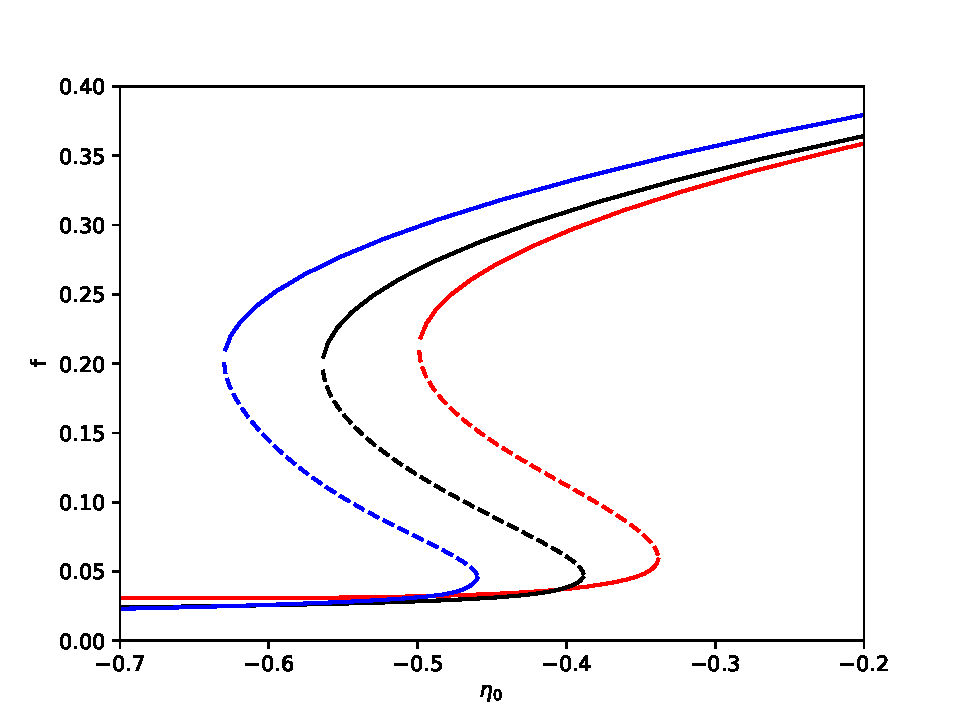
\includegraphics[width=.8\linewidth]{eta_0_continuation.pdf}
    \caption{This figure shows three continuation curves for (from left to right) $\hat{\rho}=0.55$, $\hat{\rho}=0$, and $\hat{\rho}=-0.7$.
    Using the \texttt{transform} approach, results are very well in agreement with Figure 5 in~\cite{laing2019}.
    Note that here we are using $\hat{\rho}$ and not $\rho$.}
    \label{fig:thetanet:eta_0_continuation}
\end{figure}

\subsection*{bifurcation\_tracking.py}
To reproduce Figure 6 in~\cite{laing2019} we run the following code:
\begin{lstlisting}[language=python]
import parameters as pm
import thetanet as tn
import numpy as np
from matplotlib import pyplot as plt


def main():
    # make usv_func in parameter.py available
    svd_list = np.load('svd_list.npz')
    pm.usv_func = tn.utils.usv_func_from_svd_list(svd_list)

    init_rho = -0.8
    pm.rho = init_rho
    pm.usv = pm.usv_func(pm.rho)

    b, x, stable = tn.continuation.single_param(pm)
    sn = (np.where(stable[1:] != stable[:-1])[0] + 1).tolist()

    def continue_and_plot(i):
        pm.c_ds = 0.05  # continue from init_rho to positive direction
        pm.c_steps = 130
        x_sn, y_sn = tn.continuation.saddle_node(pm, init_b=b[i], init_x=x[i], init_y=init_rho)[1:]
        plt.plot(x_sn, y_sn, c='k')

    [continue_and_plot(i) for i in sn]
    plt.axis([-0.7, -0.3, -0.8, 0.8])
    plt.xlabel(r'$\eta_0$')
    plt.ylabel(r'$\hat{\rho}$')
    plt.show()


if __name__ == '__main__':
    main()
\end{lstlisting}
The plot is shown in \autoref{fig:thetanet_bifurcation_tracking}.
\begin{figure}
    \centering
    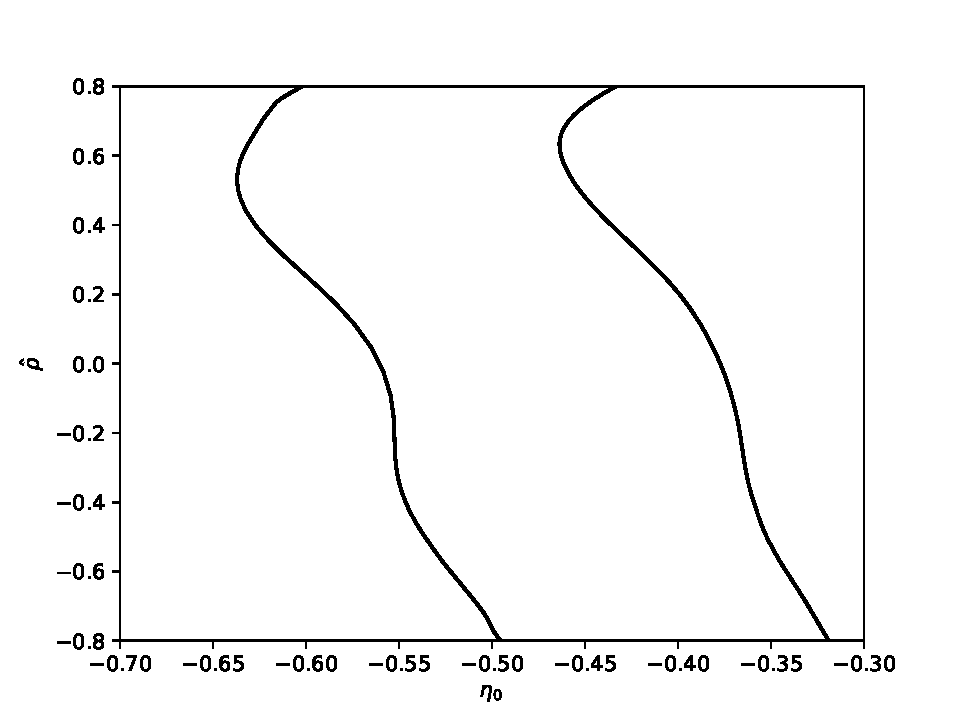
\includegraphics[width=.8\linewidth]{bifurcation_tracking.pdf}
    \caption{We find the results to be similar to Figure 6 in~\cite{laing2019}.
    Again, we are using $\hat{\rho}$ instead of $\rho$.}
    \label{fig:thetanet_bifurcation_tracking}
\end{figure}

\newpage
\bibliographystyle{alpha}
\bibliography{/home/cblasche/OneDrive/Bibliography/full_collection}
\addcontentsline{toc}{section}{References}


\end{document}
